\documentclass[11pt, a4paper]{article}
\usepackage{amsmath,amsthm, graphicx}
\usepackage{verbatim}
\usepackage{titlesec}

\titleclass{\subsubsubsection}{straight}[\subsection]

\newcounter{subsubsubsection}[subsubsection]
\renewcommand\thesubsubsubsection{\thesubsubsection.\arabic{subsubsubsection}}
\renewcommand\theparagraph{\thesubsubsubsection.\arabic{paragraph}} % optional; useful if paragraphs are to be numbered

\titleformat{\subsubsubsection}
{\normalfont\normalsize\bfseries}{\thesubsubsubsection}{1em}{}
\titlespacing*{\subsubsubsection}
{0pt}{3.25ex plus 1ex minus .2ex}{1.5ex plus .2ex}

\def\toclevel@subsubsubsection{4}
\def\l@subsubsubsection{\@dottedtocline{4}{7em}{4em}}

\title{ELEN4009 - Software Engineering\\Smart Home Power Management System\\Lab 03 - First Prototype of the Project}
\author{Ari Croock (718005)\\Kanaka Babshet (678851)\\Alice Yang (597609)\\Daniel Weinberg (547937)}
\date{\today}
\setcounter{secnumdepth}{4}
\setcounter{tocdepth}{4}

\begin{document}
	\maketitle
	\section{Introduction}
	%\subsection{Purpose}
	This report documents the implementation of the first prototype of the Smart Home Power Management System. 
	\newline
	\newline	
	\noindent
	The project aims to provide a flexible software system which is able to remotely control and monitor IoT devices, as well as perform detailed power consumption diagnostics.
		
	%\subsection{Project Scope}

	\section{Work Schedule}
	
	\subsection{Prototype development execution}
	All work was conducted as a well collaborated team. Upon receiving information complying to the deliverables of this lab, a three-hour sprint planning meeting was called in order to conclude the following: 
	\begin{enumerate}
		\item The sprint goal
		\item The action plan of how to achieve this goal by the target date (07/04/2016)
	\end{enumerate}
	\noindent
	As is required in a sprint planning meeting, the product backlog was first created in order to decide which of these tasks will be transferred to the sprint backlog for the latest product increment. 
	Upon this discussion, a sprint backlog was drawn up on Trello (a software collaboration tool). The sprint backlog is a basic list of the tasks that must be implemented by the team in order to deliver a functional product increment at the end of that sprint \cite{sprintbacklogdef}. 
	\newline
	\newline
	\noindent
	With a timebox of 2 weeks, tasks were delegated and the product was worked on and shared amongst the team using GIT, while sprint retrospective meetings were held once every week on Thursdays. Figure~\ref{fig:init_backlogs} below details the product backlog and sprint backlog created on Trello.
	\newline
	\newline
	\noindent	
	As was decided at the commencement of this project, Alice Yang and Daniel Weinberg have been assigned to the front-end development, whereas Ari Croock and Kanaka Babshet have been assigned to the back-end development. 
	\newline
	
	\begin{figure}[htb]
		\centering
		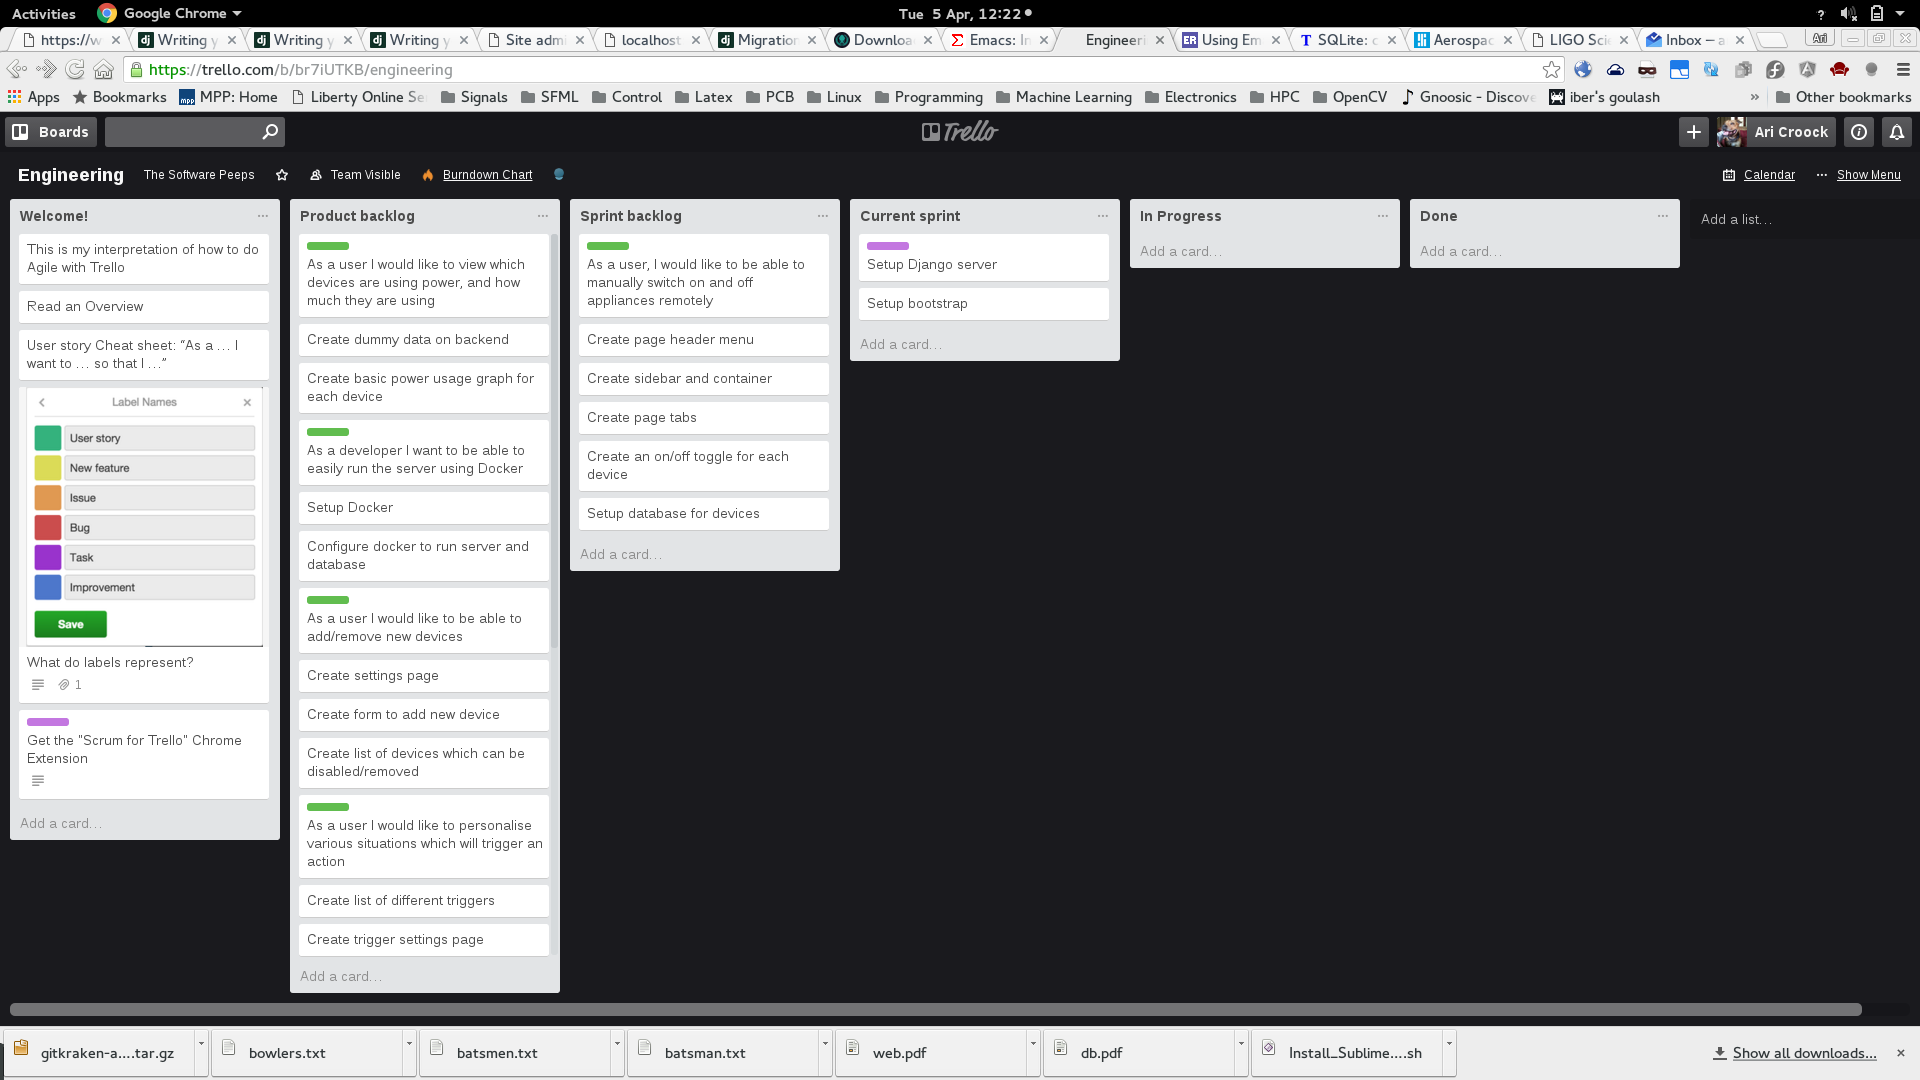
\includegraphics[width=\linewidth]{init_backlogs}
		\caption{Screenshot of the Trello page drawn on the first day of the initial prototype implementation}
		\label{fig:init_backlogs}
	\end{figure}
	%\newpage
	\subsection{Key Modules Selected for Project Illustration:}
	A few class modules have been written using Django, a high-level Python Web framework, in conjunction with Bootstrap, a powerful front-end framework, for the first prototype: 
	\begin{enumerate}
		\item A scrollable webpage, with a page header and tabs
		\item The addition and removal of a device, with corresponding specifications
		%\item Setting parameters which do not allow certain device characteristics when adding a device
		\item Viewing the devices connected
		\item Toggling between the state of devices
	\end{enumerate}
	
	\subsection{Testing:}
	Simple tests have been written and conducted along the development process of this prototype: 
	\subsubsection{Back-end:}
	\begin{enumerate}
		\item Check that a device can be added to the database
		\item Test that the system does not allow datatypes which do not fit the device specifications. For example, a user cannot enter a device IP address as "3498347", but instead it must be an IPv4 or IPv6 address. 
		\item Check that a certain home location cannot contain two devices with the same names. For example, a kitchen cannot contain "kettle 1" and "kettle 1" 
		\item Test that no two devices can have the same IP address
	\end{enumerate}
	\subsubsection{Front-end:}
	$<$Alice and Weiny add your tests here please $>$
	
\begin{thebibliography}{9}
	\bibitem{sprintbacklogdef} Luciano Felix. 2009. \textit{9 Tips for Creating a Good Sprint Backlog}. [ONLINE] Available at: https://www.scrumalliance.org/community/articles/2009/march/9-tips-for-creating-a-good-sprint-backlog. [Accessed 06 April 16].
\end{thebibliography}
		
\end{document}